% Intended LaTeX compiler: pdflatex
\documentclass[10pt,a4paper,UTF8]{article}
\usepackage{zclorg}
\author{emacsun}
\date{}
\title{使用make编译多个文件}
\hypersetup{
 pdfauthor={emacsun},
 pdftitle={使用make编译多个文件},
 pdfkeywords={},
 pdfsubject={},
 pdfcreator={Emacs 25.0.50.1 (Org mode 9.0.6)},
 pdflang={English}}
\begin{document}

\maketitle
\tableofcontents
\titlepic{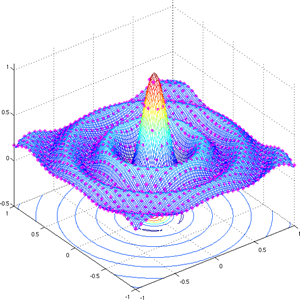
\includegraphics[scale=0.25]{../../img/sinc.PNG}}

\section{引言}
\label{sec:org8c2b8b4}


作为一名通信工程师,通常的C/C++代码都是只有一个文件,比如Turbo编码器或者译码器,LDPC编码器或者译码器。但是,偶尔也会用到需要编译多个文件的时候。我对庞大的Visual Studio又比较畏惧(主要是我那256G的硬盘比较畏惧),倾向于使用GCC。所以本文记录使用 \texttt{GCC} 和 \texttt{make} 编译多个文件。
\section{九个文件的工程}
\label{sec:org097050b}


首先给出有九个文件的工程,这九个文件分别是 \texttt{sum.c} \texttt{sum.h} \texttt{substract.c} \texttt{substract.h} \texttt{multiply.c} \texttt{multiply.h} \texttt{divide.c}  \texttt{divide.h}  \texttt{main.c} 其内容分别是实现浮点加减乘除。为节省篇幅,仅列出 \texttt{sum.h} 和 \texttt{sum.c} 。首先 \texttt{sum.h} ,这个文件只有一行,即 \texttt{sum()} 函数的声明。

\lstset{language=C,label= ,caption= ,captionpos=b,numbers=none}
\begin{lstlisting}
float sum(float a, float b);
\end{lstlisting}
然后是 \texttt{sum.c} ,这个文件实现了 \texttt{sum()} 函数。
\lstset{language=C,label= ,caption= ,captionpos=b,numbers=none}
\begin{lstlisting}
#include "sum.h"

float sum(float a, float b){
  return a + b;
}
\end{lstlisting}
主文件 \texttt{main.c} 是:
\lstset{language=C,label= ,caption= ,captionpos=b,numbers=none}
\begin{lstlisting}
#include <stdio.h>
#include <math.h>
#include "sum.h"
#include "substract.h"
#include "multiply.h"
#include "divide.h"

int main(int argc, char *argv[])
{
  float a,b;
  a = 3;
  b = 4;
  printf("%f = %f + %f\n",sum(a,b),a,b);
  printf("%f = %f - %f\n",substract(a,b),a,b);
  printf("%f = %f * %f\n",multiply(a,b),a,b);
  printf("%f = %f / %f\n",divide(a,b),a,b);

  return 0;
}
\end{lstlisting}
编译这九个文件的常规做法是逐个编译,或者使用:
\begin{verbatim}
gcc main.c sum.c substract.c multiply.c divide.c -o main
\end{verbatim}
但是这种做法的缺点是明显的:
\begin{enumerate}
\item 随着文件的增多,编译工作将是一个工作量很大的无营养工作。
\item 对于没有修改过的文件也要重新编译,无疑将增加编译时间
\end{enumerate}
\section{make}
\label{sec:orgea4c38d}


我的make是跟着陈皓学的(陈皓是著名文档《跟我一起写Makefile》的作者。对于每个严肃的make学习者,这个文档都是极佳的入门资料。)

这个工程的makefile可以写为:
\lstset{language=make,label= ,caption= ,captionpos=b,numbers=none}
\begin{lstlisting}
main: main.o sum.o substract.o multiply.o divide.o
  gcc main.o sum.o substract.o multiply.o divide.o -o main
main.o: main.c
  gcc -c main.c
sum.o: sum.c
  gcc -c sum.c
substract.o:substract.c
  gcc -c substract.c
multiply.o: multiply.c
  gcc -c multiply.c
divide.o: divide.c
  gcc -c divide.c
\end{lstlisting}
make有很多特殊的变量,使用这些变量可以编写更加简洁的makefile。但是这些变量的使用,会使得不太熟悉makefile的人读起来费劲。对于只有九个文件的小工程,我倾向于使用这种最原始直观的makefile。即使这种最原始的makefile也极大的降低了编译工作量。
\section{静态链接库}
\label{sec:org85e420d}


在实际工程中,我们希望把编好的程序打包变成库,供以后使用。windows和linux下都有两种打包后的程序:静态库和动态库。关于静态库和动态库,本文不做过多介绍。 这篇\href{http://www.cnblogs.com/LittleHann/p/3980364.html}{ 博文} 对C/C++ 跨平台交叉编译,静态库和动态库编译有比较详细的介绍。更详细的介绍见《程序员的自我修养:链接、装载与库》。

接下来,我演示如何在windows上使用gcc编译并使用静态库文件。静态库文件的编译非常简单,接着上面的工程:
\begin{verbatim}
gcc -c sum.c
\end{verbatim}
就会生成静态库文件 \texttt{sum.o} 。依次类推,生成 \texttt{substract.o} \texttt{multiply.o} \texttt{divide.o} ,然后使用 \texttt{ar} 把这些静态库打包:
\begin{verbatim}
ar rcs libmymath.a sum.o substract.o multiply.o divide.o
\end{verbatim}

编译 \texttt{main.c} 的时候就可以链接我们刚才生成的静态库,编译命令是:
\begin{verbatim}
gcc -o main main.c -L. -lmymath
\end{verbatim}

有两点需要注意:
\begin{enumerate}
\item \texttt{-L.} 告诉GCC除了默认目录外当前目录也是搜索静态库的目录。
\item \texttt{-lmymath} 告诉GCC链接的库的名字是 \texttt{mymath.a} .
\end{enumerate}
\end{document}
